\documentclass[11pt]{article}
\pdfoutput=1
\usepackage[
  margin=1.5cm,
  includefoot,
  footskip=30pt,
]{geometry}
\counterwithin{figure}{section}
\usepackage{tikz}
\usetikzlibrary{matrix, arrows}
\usepackage{amsmath,amssymb}
\usepackage{amsthm}
\usepackage{mathtools}
\usepackage{xspace}
\usepackage[noend]{algorithmic}
\usepackage[ruled,vlined]{algorithm2e}
\usepackage{url}
\usepackage{makeidx}
\usepackage{enumerate}
\usepackage{epstopdf}
\usepackage{booktabs}
\usepackage{color}
\usepackage[utf8]{inputenc}
\usepackage{thm-restate}
\usepackage{scalerel,stackengine}
\usepackage[shortlabels]{enumitem}
\usepackage{xr}
\usepackage{fancyvrb}
\usepackage{xcolor}
\usepackage{bold-extra}
\usepackage[width=474.18663pt]{caption}
\usepackage{subfigure}
\usepackage[most]{tcolorbox}
\usepackage{fvextra}
\usepackage[frozencache=true, finalizecache=false, cachedir=./minted-cache]{minted} 
\usepackage{float}
\usepackage{alltt}
\usepackage{soul}
\usepackage{fancyvrb}
\usepackage{multirow}
\usepackage[final]{hyperref}
\usepackage[bottom]{footmisc}

\usemintedstyle{vs}


\newcommand{\DV}{GPT-4\xspace}
\usepackage{listings}
\lstset{basicstyle=\ttfamily, columns=flexible, breaklines=true, mathescape=true}



\usepackage{tikz}
\usetikzlibrary{shapes,calc,positioning}

\global\setlength{\fboxsep}{0pt}


\tcbset{
  aibox/.style={
    width=474.18663pt,
    top=10pt,
    colback=white,
    colframe=black,
    colbacktitle=black,
    enhanced,
    center,
    attach boxed title to top left={yshift=-0.1in,xshift=0.15in},
    boxed title style={boxrule=0pt,colframe=white,},
  }
}
\newtcolorbox{AIbox}[2][]{aibox,title=#2,#1}


\definecolor{aigold}{RGB}{244,210, 1} 
\definecolor{aigreen}{RGB}{210,244,211} 
\newcommand{\lightgreen}[1]{\fcolorbox{aigreen}{aigreen}{\parbox{\linewidth}{#1}}}
\sethlcolor{aigreen}

\definecolor{aired}{RGB}{255,180,181} 
\newcommand{\lightred}[1]{\colorbox{aired}{\parbox{\linewidth}{#1}}}


\newtcbox{\mybox}[1][green]{on line,
arc=0pt,outer arc=0pt,colback=#1!10!white,colframe=#1!50!black,
boxsep=0pt,left=0pt,right=0pt,top=0pt,bottom=0pt,
boxrule=0pt,bottomrule=0pt,toprule=0pt}
\begin{document}
\include{contents/unicorn}

\title{%
\textbf{Sparks of Artificial General Intelligence:} \\
\textbf{Early experiments with GPT-4}}

\author{S\'ebastien Bubeck
\and Varun Chandrasekaran
\and Ronen Eldan
\and Johannes Gehrke
\and Eric Horvitz
\and Ece Kamar
\and Peter Lee
\and Yin Tat Lee
\and Yuanzhi Li
\and Scott Lundberg
\and Harsha Nori
\and Hamid Palangi
\and Marco Tulio Ribeiro
\and Yi Zhang
}

\date{Microsoft Research}

\maketitle

\input{contents/abstract}

\tableofcontents



\section{Introduction}

\begin{figure}[t]
\centering
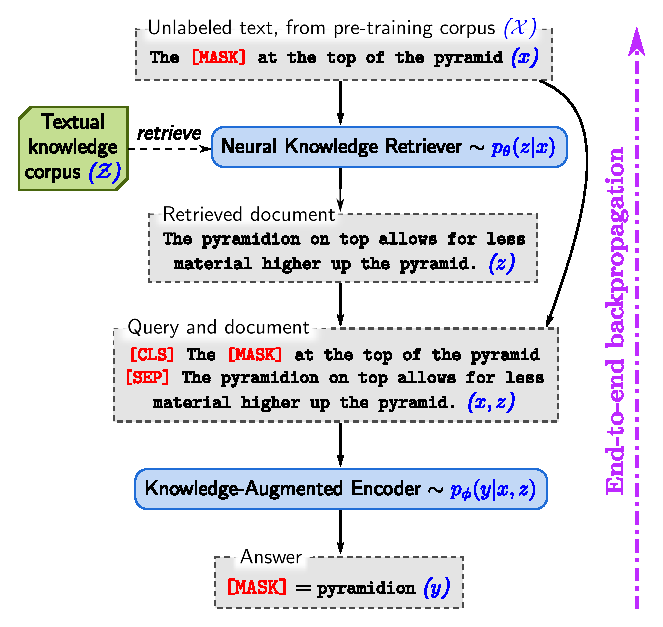
\includegraphics[width=\columnwidth]{figures/intro_end_to_end.eps}
\caption{\label{fig:intro} \ \thename augments language model pre-training with a {\bf neural knowledge retriever}
that retrieves knowledge from a {\bf textual knowledge corpus}, $\cZ$ (e.g., all of Wikipedia). Signal from the language modeling objective backpropagates all the way through the retriever, which must consider millions of documents in $\cZ$---a significant computational challenge that we address.}
\end{figure}

Recent advances in language model pre-training have shown that models such as BERT~\cite{bert}, RoBERTa~\cite{roberta} and T5~\cite{t5} store a surprising amount of world knowledge,
acquired from the massive text corpora they are trained on~\cite{lm_as_kb}.
For example, BERT is able to correctly predict the missing word in the following sentence:
\nl{The \blank\xspace is the currency of the United Kingdom} (answer: \nl{pound}).

In these language models, the learned world knowledge is stored {\em implicitly} in the parameters of the underlying neural network. This makes it difficult to determine what knowledge is stored in the network and where.
Furthermore, storage space is limited by the size of the network---to capture more world knowledge, one must train ever-larger networks, which can be prohibitively slow or expensive. 

To capture knowledge in a more interpretable and modular way, we propose a novel framework, \thefullname (\thename) pre-training, which augments language model pre-training algorithms with a learned {\em textual knowledge retriever}.
In contrast to models that store knowledge in their parameters, this approach \emph{explicitly} exposes the role of world knowledge by asking the model to decide what knowledge to retrieve and use during inference.
Before making each prediction, the language model uses the retriever to retrieve documents\footnotemark~from a large corpus such as Wikipedia,
% THE FOOTNOTE IS AT THE END TO COMBINE WITH THE RIGHT COLUMN
and then attends over those documents to help inform its prediction.
Learning this model end-to-end requires backpropagating through a retrieval step that considers an entire corpus of textual knowledge, as shown in Figure~\ref{fig:intro}.

The key intuition of \thename is to
train the retriever using a {\em performance-based} signal from unsupervised text:
a retrieval that {\em improves} the language model's perplexity is helpful and should be rewarded, while an uninformative retrieval should be penalized. 
For example, in Figure~\ref{fig:intro}, if the model needs to fill the blank in \nl{the~\blank~at the top of the pyramid}, the retriever should be rewarded for selecting a document containing \nl{The pyramidion on top allows for less material higher up the pyramid}. We achieve this behavior by modeling our {\em retrieve-then-predict} approach as a latent variable language model and optimizing the marginal likelihood.

Incorporating a large-scale neural retrieval module
during pre-training constitutes a significant computational challenge, %for pre-training,
since the retriever must consider millions of candidate documents for each pre-training step, and we must backpropagate through its decisions. To address this, we structure the retriever such that the computation performed for each document can be cached and asynchronously updated, and selection of the best documents can be formulated as Maximum Inner Product Search (MIPS).

Numerous prior works have
demonstrated the benefit of adding a discrete retrieval step to neural networks~\cite{key_value_memorynetwork, drqa}, but did not apply the framework
to language model pre-training and employed non-learned retrievers to handle large-scale document collections.
In the language modeling literature, the $k$-Nearest Neighbor Language Model~\cite{knnlm} ($k$NN-LM) retrieves similar LM examples to improve memorization. However, $k$NN-LM was not fine-tuned for downstream tasks, perhaps because it is unclear how to adapt the retrieval mechanism: a $k$NN can only use examples labeled for the target task---during fine-tuning, this precludes LM examples, which contain the desired world knowledge. In contrast, \thename's retriever is designed to transfer to other tasks, and the retrieval is just text, not a labeled example.

We evaluate our approach by fine-tuning the models pre-trained with \thename on the task of Open-domain Question Answering (\openqa), one of the most knowledge-intensive tasks in natural language processing.
%
We evaluate on three popular \openqa benchmarks (\nq, \wq, and \trec) and compare to state-of-the-art \openqa models, including both extremely large models that store knowledge implicitly (such as T5) as well as previous approaches that also use a knowledge retriever to access external knowledge, but implement retrieval in a more heuristic fashion~\cite{orqa,openqa_hardem,rrp_salesforce}. \thename achieves new state-of-the-art results on all three benchmarks, significantly outperforming all previous systems by 4-16\% absolute accuracy. We also demonstrate qualitative benefits of \thename, including interpretability and modularity.

\footnotetext{We use the term ``document'' loosely to refer to a passage from the knowledge corpus, not necessarily a whole article.}

\clearpage
\include{contents/2_see}

\clearpage
\newpage
\section{Coding}
\label{sec:code}
\vspace{-3mm}
In this section, we show that \DV\ is able to code at a very high level, both in terms of writing code from instructions and understanding existing code. \DV\ can handle a wide range of coding tasks, from coding challenges to real world applications, from low-level assembly to high-level frameworks, from simple data structures to complex programs such as games. \DV\ can also reason about code execution, simulate the effects of instructions, and explain the results in natural language. \DV\ can even execute pseudocode, which requires interpreting informal and vague expressions that are not valid in any programming language.

In its current state, we believe that \DV\ \textit{has a high proficiency in writing focused programs that only depend on existing public libraries, which favorably compares to the average software engineer's ability}. More importantly, it empowers both engineers and non-skilled users, as it makes it easy to write, edit, and understand programs. We also acknowledge that \DV\ is not perfect in coding yet, as it sometimes produces syntactically invalid or semantically incorrect code%
, especially for longer or more complex programs. \DV\ also sometimes fails to understand or follow the instructions, or produces code that does not match the intended functionality or style. 
With this acknowledgment, we also point out that \DV\ is able to improve its code by responding to both human feedback (e.g., by iteratively refining a plot in~\ref{fig:pyplot}) and compiler / terminal errors (examples in Section~\ref{sec:affordances}).
\vspace{-4mm}
\paragraph{Important Disclaimer:} As explained in the Introduction (see footnote 1 for example) our experiments were run on an early version of GPT-4. In particular all quantitative results will be different on the final version of GPT-4, although the general trends remain the same. We provide numbers here for illustration purpose only, the definitive benchmark results can be found in OpenAI's technical report \cite{gpt4}.
\vspace{-2mm}



\vspace{-1mm}
\subsection{From instructions to code}
\vspace{-1mm}
\subsubsection{Coding challenges}
\vspace{-2mm}
A common way to measure coding skill is to pose coding challenges that require implementing a specific functionality or algorithm.
We first benchmark \DV\ on HumanEval~\cite{humaneval}, a docstring-to-code dataset consisting of 164 coding problems that test various aspects of programming logic and proficiency.
As shown in Table~\ref{tab:humaneval}, \DV\ outperforms other LLMs, including \texttt{text-davinci-003} (the base model of ChatGPT) and other models trained specifically on code, \texttt{code-davinci-002}, and CODEGEN-16B~\cite{codegen}.
\vspace{-4mm}
\begin{table}[H]
\begin{center}
 \begin{tabular}{c|cccc}
\toprule
Model& \textbf{\DV} & \texttt{text-davinci-003} & Codex(\texttt{code-davinci-002}) & CODEGEN-16B \\
\midrule
\midrule
Accuracy& \textbf{82\%} & 65\% & 39\% & 30\% \\
\bottomrule
\end{tabular}
\end{center}
\vspace{-.6cm}
\caption{Zero-shot pass$@1$ accuracy comparison of different models on HumanEval}
\label{tab:humaneval}
\vspace{-3mm}
\end{table}


Although {\DV}'s accuracy shows a big jump compared to previous models, it could be that \DV\ has seen and memorized some (or all) of HumanEval during pre-training. To account for this possibility, we also evaluate it on LeetCode (\texttt{https://leetcode.com}), a popular platform for software engineering interviews, where new problems are constantly posted and updated.
We used LeetCode in Figure~\ref{fig:hired} in the introduction, where \DV\ passes all stages of mock interviews for major tech companies.
Here, to test on \emph{fresh} questions, we construct a benchmark of 100 LeetCode problems posted after October 8th, 2022, which is after \DV's pretraining period.
As seen in the example in Figure~\ref{fig:leetcode}, we paste the problem instructions into a prompt, ask \DV\ to write a python function, and use the official LeetCode online judge to check for correctness.
We present the results in Table~\ref{tab:leetcode-results}, where we compare \DV\ to other models and to human performance based on LeetCode contest results (users who fail all questions are not included, and thus this is a strong sample of humans).
We report both pass@1 and pass@5 accuracies, which measure whether the model produces a correct solution in the first or in the first five attempts, respectively. 
\DV\ significantly outperforms the other models, and is comparable to human performance (which we measure in Appendix~\ref{sec:leetcode-human}).

\vspace{-3mm}
\begin{table}[H]
\begin{center}
\begin{tabular}{l|c|c|c|c|c|c||c|c}
\toprule
  & \multicolumn{2}{c|}{Easy} &  \multicolumn{2}{c|}{Median} &  \multicolumn{2}{c||}{Hard} & \multicolumn{2}{c}{Overall}\\
\hline
pass@$k$  & $k=1$ & $k=5$ & $k=1$ & $k=5$ & $k=1$ & $k=5$ & $k=1$ & $k=5$\\
\hline
\textbf{\DV}              & \textbf{68.2} & \textbf{86.4} & \textbf{40.0} & \textbf{60.0} & \textbf{10.7} & \textbf{14.3} & \textbf{38.0} & \textbf{53.0}\\
\texttt{text-davinci-003} & 50.0 & 81.8 & 16.0 & 34.0 &  0.0 &  3.6 & 19.0 & 36.0\\
Codex (\texttt{code-davinci-002}) & 27.3 & 50.0 &  12.0 & 22.0 &  3.6 &  3.6 &  13.0 & 23.0\\
\hline
Human (LeetCode users) & \multicolumn{2}{c|}{72.2} & \multicolumn{2}{c|}{37.7} & \multicolumn{2}{c||}{7.0} & \multicolumn{2}{c}{38.2} \\
\bottomrule
\end{tabular}
\end{center}
\vspace{-6mm}
\caption{Zero-shot pass@1 and pass@5 accuracies (\%) on LeetCode.}
\label{tab:leetcode-results}
\end{table}



\begin{figure}[H]
\begin{AIbox}{\DV}
{\bf{Prompt:}}
\begin{minted}[breaklines, breaksymbol=, baselinestretch=1, fontsize=\tiny]{latex}
You are given a **0-indexed** `m x n` integer matrix `grid` and an integer `k`. You are currently at position `(0, 0)` and you want to reach position `(m - 1, n - 1)` moving only **down** or **right**.
Return *the number of paths where the sum of the elements on the path is divisible by* `k`. Since the answer may be very large, return it **modulo** `10**9 + 7`.
**Example 1:**
    Input: grid = [[5,2,4],[3,0,5],[0,7,2]], k = 3
    Output: 2
    Explanation: There are two paths where the sum of the elements on the path is divisible by k. The first path highlighted in red has a sum of 5 + 2 + 4 + 5 + 2 = 18 which is divisible by 3. The second path highlighted in blue has a sum of 5 + 3 + 0 + 5 + 2 = 15 which is divisible by 3.
**Example 2:**
    Input: grid = [[0,0]], k = 5
    Output: 1
    Explanation: The path highlighted in red has a sum of 0 + 0 = 0 which is divisible by 5.
**Constraints:**
-  `m == grid.length`
-  `n == grid[i].length`
-  `1 <= m, n <= 5 * 10**4`
-  `1 <= m * n <= 5 * 10**4`
-  `0 <= grid[i][j] <= 100`
-  `1 <= k <= 50`
**Hints:**
-  The actual numbers in grid do not matter. What matters are the remainders you get when you divide the numbers by k.
-  We can use dynamic programming to solve this problem. What can we use as states?
-  Let dp[i][j][value] represent the number of paths where the sum of the elements on the path has a remainder of value when divided by k.
\end{minted}


{\bf \DV:}
\vspace{-0.1cm}
\begin{minted}[breaklines, breaksymbol=, baselinestretch=1, fontsize=\tiny]{python}
class Solution(object):
    def numberOfPaths(self, grid, k):
        """
        :type grid: List[List[int]]
        :type k: int
        :rtype: int
        """
        # Define MOD as 10**9 + 7
        MOD = 10**9 + 7
        # Get the dimensions of the grid
        m = len(grid)
        n = len(grid[0])
        # Initialize a 3D dp array with all zeros
        # dp[i][j][value] represents the number of paths where the sum of the elements on the path has a remainder of value when divided by k
        dp = [[[0] * k for _ in range(n)] for _ in range(m)]
        # Base case: the first cell has only one path and its value is grid[0][0] %
        dp[0][0][grid[0][0] %
        # Loop through the grid
        for i in range(m):
            for j in range(n):
                # Skip the first cell
                if i == 0 and j == 0:
                    continue
                # Loop through all possible remainders
                for value in range(k):
                    # The number of paths to the current cell with the current remainder is equal to the sum of:
                    # - The number of paths to the top cell with the previous remainder
                    # - The number of paths to the left cell with the previous remainder
                    # The previous remainder is equal to the current remainder minus the current value, plus k if it is negative
                    prev = (value - grid[i][j]) %
                    if i > 0:
                        dp[i][j][value] += dp[i - 1][j][prev]
                    if j > 0:
                        dp[i][j][value] += dp[i][j - 1][prev]
                    # Take the modulo to avoid overflow
                    dp[i][j][value] %
        # Return the number of paths to the bottom right cell with a remainder of 0
        return dp[m - 1][n - 1][0]
\end{minted}

\end{AIbox}
\caption{Solving a LeetCode problem using dynamic programming. \DV's solution also has better readability thanks to comprehensive commenting.}
\label{fig:leetcode}
\end{figure}












\subsubsection{Real world scenarios}
Coding challenges can evaluate the skills in algorithms and data structures. However, they often fail to capture the full complexity and diversity of real-world coding tasks, which requires specialized domain knowledge, creativity, and integration of multiple components and libraries, as well as the ability to change existing code. 
To assess \DV's ability to code in more realistic settings, we design end-to-end real-world coding challenges related to data visualization, \LaTeX\ coding, front-end development, and deep learning, each of which requires different specialized skills.
For each task, we provide \DV\ with high-level instructions, ask it to write the code in the appropriate language and framework. In a few cases, we also change the specification \emph{after} the code is written and ask for an update.

\paragraph{Data Visualization} %
In Figure~\ref{fig:pyplot}, we ask both \DV{} and ChatGPT to extract data from the \LaTeX\ code for Table~\ref{tab:leetcode-results} and produce a plot in Python based on a conversation with the user. Afterwards, we ask both models to perform various operations on the produced plots. While both models extract the data correctly (not a trivial task, since one must infer from the multicolumn that the Human row has the same value for $k=1$ and $k=5$), ChatGPT never produces the desired plot. In contrast, \DV{} responds appropriately to all user requests, manipulating the data into the right format and adapting the visualization. In Appendix~\ref{sec:imdb}, we include another example where \DV visualizes the IMDb dataset.
\begin{figure}[H]
\centering
\begin{AIbox}{\DV}
\centering
\begin{tikzpicture}
\matrix (m) [matrix of nodes, column sep=0cm, row sep=0.1cm] {
  \includegraphics[width=0.6\linewidth, height=0.3\linewidth]{figures/DV3_plot_1.png} \\
  \includegraphics[width=0.6\linewidth, height=0.3\linewidth]{figures/DV3_plot_2.png} \\
  \includegraphics[width=0.6\linewidth, height=0.3\linewidth]{figures/DV3_plot_3.png} \\
};

\node [left=0.2cm of m-1-1, text width=0.35\linewidth, align=left, anchor=east, yshift=-1] (start) 
{{\bf Prompt: }\\
{\scriptsize [in an interactive manner]}
\\
\hfill \break
\scriptsize\texttt{I will show you a LaTeX table, and we will come up with a way to visualize it better in a question and answer format
The table is showing the performance of different language models (and human users) in generating solutions to code challenges. Pass@1 means the first generation works, while Pass@5 means one out of 5 generation works...}};

\draw [-triangle 90] (start) to ([xshift=0.1cm]m-1-1.west);

\draw [-triangle 90, bend right=30, thick] ([yshift=-2cm]m-1-1.west) to node [left, text width=0.35\linewidth, align=left, yshift=-1cm] 
{\scriptsize \texttt{Can you make both plots have the same range in the y axis? And the legend has each model name twice.}} ([yshift=-1cm]m-2-1.west);

\draw [-triangle 90, bend right=30, thick] ([yshift=-2cm]m-2-1.west) to node [left, text width=0.35\linewidth, align=left, yshift=-1cm] 
{\scriptsize \texttt{Is there a way to make the `Human' bar more distinctive, to separate it from the other 3?}} ([yshift=-1cm]m-3-1.west);
\end{tikzpicture}
\end{AIbox}
\caption{\DV visualizes data from a \LaTeX\ table (i.e., Table~\ref{tab:leetcode-results}). We point out that \DV also generates the format for this figure. We asked the model how to plot arrows connecting figures in \LaTeX\, and \DV produced a working Tikz snippet with the layout and arrows that we adopt here.}
\label{fig:pyplot}
\end{figure}






\paragraph{Front-end / Game development}
In Figure~\ref{fig:games}, we ask \DV\ to write a 3D game in HTML with JavaScript, using a very high-level specification. \DV\ produces a working game in \textbf{zero-shot} fashion that meets all the requirements. In the 3D game, \DV{} is even able to interpret the meaning of ``defender avatar is trying to block the enemy'': the defender code has logic so that it positions itself between the player and enemy. In contrast, ChatGPT responds with ``I am an AI language model, I can provide you guidance on how to create a 3D game in HTML with JavaScript, but I am unable to write code or create a game myself.
Creating a 3D game in HTML with JavaScript requires a lot of programming knowledge and experience. It is not a task that can be completed quickly or easily. It would take a significant amount of time and effort to develop all the necessary features, such as 3D graphics, physics, user input, and AI...''. We give more examples for front-end (graphical user interface) and game development in Appendix~\ref{sec:code_appendix}. 


\begin{figure}[H]
\begin{AIbox}{\DV}
{\bf Prompt:}
\vspace{-0.3cm}
\begin{minted}[breaklines, breaksymbol=, baselinestretch=1, fontsize=\tiny]{html}
Can you write a 3D game in HTML with Javascript, I want:
-There are three avatars, each is a sphere.
-The player controls its avatar using arrow keys to move.
-The enemy avatar is trying to catch the player.
-The defender avatar is trying to block the enemy.
-There are also random obstacles as cubes spawned randomly at the beginning and moving randomly. The avatars cannot cross those cubes.
-The player moves on a 2D plane surrounded by walls that he cannot cross. The wall should cover the boundary of the entire plane. 
-Add physics to the environment using cannon.
-If the enemy catches the player, the game is over.
-Plot the trajectories of all the three avatars.
\end{minted}
\begin{subfigure}
\centering
\captionsetup{width=1\linewidth}
\includegraphics[width=1\linewidth]{figures/3d_game_run_1.png}
\caption*{\scriptsize {\bf Episode 1:} the player avatar (\textcolor{blue}{blue}) stands still. The enemy (\textcolor{red}{red}) rushes straight towards the player, while the defender (\textcolor{magenta}{magenta}) attempts to `body block' the enemy (see its curved trajectory in \textcolor{magenta}{magenta}).}
\end{subfigure}
\hfill
\begin{subfigure}
\centering
\captionsetup{width=1\linewidth}
\includegraphics[width=1\linewidth]{figures/3d_game_run_2.png}
\caption*{\scriptsize {\bf Episode 2:} the player (\textcolor{blue}{blue}) wanders around. The enemy (\textcolor{red}{red}) attempts to close the gap but crashes into a cube and bounces into the air. Trying to obstruct, the defender (\textcolor{magenta}{magenta}) mimics its move to follow up into the air, but ends up failing. The enemy (\textcolor{red}{red}) catches the player (\textcolor{blue}{blue}) in the end.}
\end{subfigure}
\end{AIbox}
\caption{\DV~ develops a complex 3D HTML game in JavaScript.}
\label{fig:games}
\end{figure}


\paragraph{Deep Learning.}
Writing code for deep learning requires knowledge of mathematics, statistics, and familiarity with frameworks and libraries such as PyTorch, TensorFlow, Keras, etc. 
In Figure~\ref{fig:deeplearning} we ask both \DV\ and ChatGPT to write a custom optimizer module, a task that can be challenging and error-prone even for human deep learning experts. We give these models a natural language description, which includes a sequence of non-trivial operations such as applying SVD, truncating a matrix spectrally at the top-k and top-2k eigenvalues, normalizing the top-k truncated matrix using the F-norm of the top-2k truncated matrix, applying momentum and weight decay.
These instructions are not spelled out in complete detail, e.g., ``apply momentum on $G_k$'' requires ``deep learning common sense''.
It is important to note that this particular optimizer does not exist in the literature or on the internet, and thus the models cannot have it memorized, and must instead compose the concepts correctly in order to produce the code. 









\begin{figure}[H]
\begin{AIbox}{\DV~vs ChatGPT}
{\bf Prompt:}
\begin{minted}[breaklines, breaksymbol=, baselinestretch=1, fontsize=\tiny]{html}
I want to write a customized optimizer in pytorch, the optimizer should do:
1. the parameters for the optimizer is learning rate, momentum ,weigth decay, d_dim, k and factor alpha
2. the optimizer goes through each parameter in the network, and then
-- Get the gradient of this parameter, reshape it to 2D by looping through the dimensions, and keeping the dimension whose actual dimension (shape) is equal to d_dim, do an SVD decomposition of the parameter so G = U\Sigma V. 
-- Keep the top k singular vectors of G, so we get a new matrix G_k = U \Sigma_k V. 
-- Keep the top 2k singular vectors of G, so we get a new matrix G_{2k} = U \Sigma_{2k} V. 
-- Normalize G_k according to the momentum of the F-norm of G_{2k}.
-- Truncate each coordinate of G_k to the top alpha  percentile of all the coordinates, in absolute value.
-- Apply momentum on G_k, and then update the network parameters using this momentum.
-- Apply weight decay.
\end{minted}
\begin{minipage}[t]{0.5\linewidth}
{\bf \DV:}
\begin{minted}[breaklines, breaksymbol=, baselinestretch=1, fontsize=\tiny, highlightlines={20-23}, highlightcolor=aigold]{python}
def step(self):
    for group in self.param_groups:
        for p in group['params']:
            if p.grad is None:
                continue
            grad = p.grad.data
            # reshape grad to 2D
            grad_2d = grad.reshape(-1, group['d_dim'])
            # SVD decomposition
            U, S, V = torch.svd(grad_2d)
            # keep top k singular vectors
            G_k = U[:, :group['k']] @ torch.diag(S[:group['k']]) @ V[:, :group['k']].T
            # keep top 2k singular vectors
            G_2k = U[:, :2*group['k']] @ torch.diag(S[:2*group['k']]) @ V[:, :2*group['k']].T
            # normalize G_k 
            G_k /= torch.norm(G_2k, p=2)
            # truncate G_k 
            threshold = torch.quantile(torch.abs(G_k), group['alpha'])
            G_k[torch.abs(G_k) < threshold] = 0
            # apply momentum
            if 'momentum_buffer' not in group:
                group['momentum_buffer'] = torch.zeros_like(G_k)
            group['momentum_buffer'] = group['momentum'] * group['momentum_buffer'] + G_k 
            # update parameters
            p.data.add_(-group['lr'] * group['momentum_buffer'])
            # apply weight decay
            if group['weight_decay'] != 0:
                p.data.add_(-group['weight_decay'] * group['lr'], p.data)
\end{minted}
\end{minipage}
\begin{minipage}[t]{0.5\linewidth}
{\bf ChatGPT:}
\begin{minted}[breaklines, breaksymbol=, baselinestretch=1, fontsize=\tiny, highlightlines={24}, highlightcolor=aired]{python}
def step(self):
    for group in self.param_groups:
        for p in group['params']:
            if p.grad is None:
                continue
            grad = p.grad.data
            grad = grad.reshape(-1, grad.shape[-1]) # reshape to 2D
            
            # SVD decomposition
            u, s, v = torch.svd(grad)
            
            # Keep top k and 2k singular vectors
            k = group['k']
            u_k = u[:,:k]
            s_k = s[:k]
            v_k = v[:,:k]
            u_2k = u[:,:2*k]
            s_2k = s[:2*k]
            v_2k = v[:,:2*k]
            
            # Normalize according to momentum of F-norm of G_2k
            grad_k = u_k @ torch.diag(s_k) @ v_k.t()
            norm_2k = s_2k.norm()
            grad_k = grad_k * group['momentum'] / norm_2k
            
            # Truncate to top alpha percentile
            alpha = group['alpha']
            percentile = grad_k.abs().flatten().kthvalue(int(alpha * grad_k.numel()))
            grad_k[grad_k.abs() < percentile] = 0
            
            # Apply weight decay
            p.data.add_(-group['lr'], grad_k + group['weight_decay'] * p.data)
\end{minted}
\end{minipage}
\end{AIbox}
\caption{\DV~vs ChatGPT at implementing a customized Pytorch optimizer module. We highlight the \fcolorbox{aigold}{aigold}{astuteness} of \DV vs the \fcolorbox{aired}{aired}{mistake} by ChatGPT at `applying momentum'. }
\label{fig:deeplearning}
\end{figure}


While both models produce syntactically valid code, only \DV's response largely matches the instructions, while it forgets to `loop through the dimensions' and to `normalize $G_k$ according to the momentum' where the instructions happen to be particularly vague. In comparison, ChatGPT makes a rather fatal mistake at applying momentum (highlighted in red) in addition. Note that applying momentum in PyTorch is a non-trivial task that requires storing and reading a moving average into and from a separate state buffer.


\paragraph{Interfacing with \LaTeX.} Writing in \LaTeX\ is an important exercise for computer scientists and mathematicians but has a non-trivial learning curve. Even experts make irritating errors that take hours to fix on a daily basis due to its strict grammar and the lack of a good debugger. We show that {\DV} can utilize its master-level \LaTeX\ coding skill to greatly simplify the process, with the potential of serving as a new generation of \LaTeX\ compilers that can handle imprecise natural language descriptions. In~Figure~\ref{fig:code-LaTeX}, we ask {\DV} to transfer a snippet of written in a semi-rigorous (buggy) \LaTeX\ code mixed with natural language into accurate \LaTeX\ commands that compiles and is faithful in one shot. In constrast, ChatGPT generates a snippet that does not compile due to mistakes at using `\#' and `\textbackslash{color}' etc.

\begin{figure}[H]
\begin{AIbox}{\DV vs ChatGPT}
{\bf Prompt:}
\begin{minted}[breaklines, breaksymbol=, baselinestretch=1, fontsize=\tiny]{html}
A function f is called {increasing}_{emphasize!} if f(s) <= f(t) holds for every s <= t. Consider the formula:
limit_{x goes to 0} {limit when n approaches infinite} underscore{ 
\matrix[ [ sum of i from 1 to n (f(nx) - integral from 0 to x sin(nx) dx ),  
((x + 2/8)^2 - 5)/((4x-1/x^2) /(n xor 3)), \\ , ..., partial f(x/n)
over partial x * (e^{-i*omega n x} + 3(x#7) ) , f inverse of (x mod n) ]]
multiply \matrix{1, 1, ..., 1 \\ 1, 1, ..., 1} }
{grey_color{this gives us a good impression about the function}}

Convert the above paragraph to LaTeX.
\end{minted}

\parbox[t]{\linewidth}{{\bf \DV:}\\\scriptsize
A function $f$ is called \emph{increasing} if $f(s) \leq f(t)$ holds for every $s \leq t$. Consider the formula:
\[
\lim_{x \to 0} \lim_{n \to \infty} \underbrace{ \begin{bmatrix} \sum_{i = 1}^n \left(f(nx) - \int_0^x \sin(nx) \, dx \right), & \frac{\left(x + \frac{2}{8}\right)^2 - 5}{\frac{4x-1/x^2}{n \oplus 3}}, \\ \vdots & \vdots \\ \frac{\partial f(x/n)}{\partial x} \cdot  \left(e^{-i \omega n x} + 3(x\#7) \right), & f^{-1} (x \bmod n) \end{bmatrix}  \times  \begin{bmatrix} 1 & 1 & \cdots & 1 \\ 1 & 1 & \cdots & 1 \end{bmatrix} }_{\textcolor{gray}{\text{this gives us a good impression about the function}}}
\]}\\
{\bf ChatGPT:}
\begin{minted}[breaklines, breaksymbol=, baselinestretch=1, fontsize=\scriptsize]{html}
A function $f$ is called {\em increasing} if $f(s) \leq f(t)$ holds for every $s \leq t$. Consider the formula:
$$\lim_{x \to 0} \lim_{n \to \infty} \begin{bmatrix} \sum\limits_{i=1}^{n} (f(nx) - \int\limits_0^x \sin(nx),dx), \ \frac{(\frac{x}{2} + \frac{1}{8})^2 - 5}{\frac{4x - \frac{1}{x^2}}{n \operatorname{xor} 3}}, \ \vdots, \ \frac{\partial f(x/n)}{\partial x} \cdot (e^{-i\omega n x} + 3(x#7)), \ f^{-1}(x \bmod n) \end{bmatrix} \cdot \begin{bmatrix} 1 \ 1 \ \vdots \ 1 \end{bmatrix}$$
{\color{grey}This gives us a good impression about the function.} \]
\end{minted}
\end{AIbox}
\caption{\DV translates semi-rigorous typesetting instructions into a working \LaTeX\ snippet. For \DV we present the final graphic, while ChatGPT's generation fails to compile. }
\label{fig:code-LaTeX}
\end{figure}

\subsection{Understanding existing code}
The previous examples have shown that \DV\ can write code from instructions, even when the instructions are vague, incomplete, or require domain knowledge. They also showed that \DV\ could respond to follow-up requests, modifying its own code according to instructions.
However, another important aspect of coding is the ability to understand and reason about existing code, written by others, which might be complex, obscure, or poorly documented. 
To test this we pose various questions that require reading, interpreting, or executing code written in different languages and paradigms.

\paragraph{Reverse-engineering assembly code.}
Reverse engineering is an essential test for software security which amounts to search for useful information in a executable program written in a machine-readable (i.e., binary) representation of CPU instructions. It is a challenging task that requires understanding the syntax, semantics, and conventions of assembly language, as well as the architecture and behavior of the processor and the operating system. 

We task \DV\ with performing penetration testing on a binary executable file (code was written in C) that requires a password to run. We do this via a chat format, where \DV\ tells the user which commands to run, and the user responds with the results. We also show in Section~\ref{sec:affordances} that \DV\ is able to run a shell independently, but this chat mode also provided the benefit of it explaining every step. \DV\ checks the file format and metadata, disassembles the code with tools like ``objdump'' and ``radare2'', debugs the code with ``gdb'' and ``ltrace'', and reverse engineers it with techniques like patching, hooking, and decompiling. During this process, \DV\ figures out that from the assembly code that the password is compared to a hash value derived from a simple mathematical formula. \DV\ then writes a python program that tries different combinations of numbers until it finds one that matches the hash value, cracking the password (an abbreviated log is presented in Appendix~\ref{appendix:reverse-engine}). ChatGPT refuses to do it on the grounds of it being illegal and unethical, even though reverse engineering is a common practice to \emph{ensure} software security. Moreover, \DV exhibits all-around proficiency in utilizing existing tools also beyond programming, which we will discuss in details in Section~\ref{sec:affordances}.


\paragraph{Reasoning about code execution.}
In the example in Figure~\ref{fig:code-memory-align}, we ask \DV and ChatGPT to predict and explain the output of a C program that prints the size of two structures. \DV correctly explains that the output may vary depending on the alignment rule used by the compiler, and gives an example of a possible output with 4-byte alignment. ChatGPT ignores the alignment issue and gives a wrong output, and also makes a false statement about the order of the members not affecting the size of the structure.

\begin{figure}[H]
\begin{AIbox}{\DV~vs ChatGPT}

{\bf Prompt:}  


 \begin{minted}[breaklines, breaksymbol=, baselinestretch=1, fontsize=\scriptsize]{cpp}
struct mystruct_A {  char a; int b; char c; } x;
struct mystruct_B {  int b;  char a; char c; } y;
    
#include <stdio.h>
int main(void) {
    printf("Size of x: %
    printf("Size of y: %
    return 0;
}
    
Possible Output:
\end{minted}   

\parbox[t]{0.53\linewidth}{{\bf \DV:} 
\tiny
\begin{alltt}
There are different ways to implement and align structures in memory, so the exact output may vary depending on the compiler, platform, and options used. However, one possible output is:\\

Size of x: 12 bytes\\
Size of y: 8 bytes\\

This output assumes that the compiler uses 4-byte alignment for structures, meaning that each structure member starts at an offset that is a multiple of 4 bytes from the beginning of the structure. This may result in some padding bytes being inserted between or after the members to maintain alignment. For example, 
\fcolorbox{aigold}{aigold}{in x, there may be 3 padding bytes after a and 3 padding bytes after c,}
\fcolorbox{aigold}{aigold}{while in y, there may be no padding at all.} 
The size of a structure is the sum of the sizes of its members plus any padding bytes.
\end{alltt}
}\hspace{0.02\linewidth}%
\parbox[t]{0.45\linewidth}{{\bf ChatGPT:}
\tiny
\begin{alltt}
Size of x: 8 bytes\\
Size of y: 8 bytes\\

The output of this code would be the size of the two structures in bytes. The size of a structure in C is the sum of the sizes of all of its members. In this case, the size of mystruct\textunderscore A is the size of a char plus the size of an int plus the size of another char, which is \fcolorbox{aired}{aired}{1 + 4 + 1 = 8} bytes. \\
\\
Similarly, the size of mystruct\textunderscore B is also 8 bytes. This means that both structures will be allocated the same amount of memory. \\
\\
\fcolorbox{aired}{aired}{Note that the order in which the members are}
\fcolorbox{aired}{aired}{declared in the structure does not affect its}
\fcolorbox{aired}{aired}{size.}
\end{alltt}
}
\end{AIbox}
\caption{\DV vs ChatGPT on the~memory alignment rule of C/C\texttt{++}. \DV's insightful comments are labeled in \fcolorbox{aigold}{aigold}{gold} and ChatGPT's Mistakes are labeled in \fcolorbox{aired}{aired}{red}.}
\label{fig:code-memory-align}
\end{figure}


\paragraph{Executing Python code} The ultimate test of understanding the existing code is to ask the model to directly execute it. 
In Figure~\ref{figure:pseudo1}, we see that \DV{} is able to execute non-trivial Python code. It has to keep track of several variables (including a nested loop and a dictionary) and deal with recursion. It explains the execution in detail by writing intermediate steps and comments. It is important to note that \DV{} is not running the code on a Python interpreter, but rather simulating the code in natural language. This requires a high level of understanding and reasoning about the code, as well as the ability to communicate the results clearly. In contrast, ChatGPT states (incorrectly) that ``The result of DP(3, 4) is not specified in the given code'', and later on that ``It is not clear from the code what the expected output of the function is, as the specific problem that the function is solving is not provided.'' ChatGPT does not simulate the full execution, but states which functions will be called. %
\begin{figure}[H]
\begin{AIbox}{\DV vs ChatGPT}
\begin{minipage}[t]{0.15\linewidth}
{\bf Prompt:}
\end{minipage}
\begin{minipage}[t]{0.8\linewidth}
{\tiny
I have the following python code:}
\vspace{-0.1cm}
\begin{minted}[breaklines, breaksymbol=, baselinestretch=1, fontsize=\tiny]{python}
def to_str(i, j):
    return str(i) + "," + str(j)
dict = {}
def DP(i, j):
    if i <= 0 or j <= 0:
        dict[to_str(i, j)] = abs(4 * j - 3 * i) 
    elif to_str(i, j) not in dict.keys():
        arr = []
        for ir in range(i):
            for jr in range(j):
                arr.append(DP(ir, jr))
        dict[to_str(i, j)] = max(arr)
    return dict[to_str(i, j)]
\end{minted}
\vspace{-0.5cm}
{\tiny What is the result of DP(3, 4)? Write down the execution with intermediate steps.}\\
\end{minipage}
\vspace{-0.5cm}

{\bf\DV:}
\vspace{-0.1cm}
\begin{minted}[breaklines, breaksymbol=,  fontsize=\tiny]{html}
DP(3, 4):
- i > 0 and j > 0, so we don't return from the first if statement
- to_str(3, 4) is not in dict, so we enter the second if statement
- arr = []
- We loop through ir from 0 to 2, and jr from 0 to 3
  - to_str(0, 0)  is not in dict, so DP(0, 0) returns abs(4 * 0 - 3 * 0) = 0, dict =  {"0,0": 0}, arr = [0]
  - to_str(0, 1)  is not in dict, so DP(0, 1) returns abs(4 * 1 - 3 * 0) = 4, dict =  {"0,0": 0, "0,1": 4}, arr = [0, 4]
  - to_str(0, 2)  is not in dict, so DP(0, 2) returns abs(4 * 2 - 3 * 0) = 8, dict =  {"0,0": 0, "0,1": 4, "0,2": 8}, arr = [0, 4, 8]
  - to_str(0, 3)  is not in dict, so DP(0, 3) returns abs(4 * 3 - 3 * 0) = 12, dict =  {"0,0": 0, "0,1": 4, "0,2": 8, "0,3": 12}, arr = [0, 4, 8, 12]
  - to_str(1, 0)  is not in dict, so DP(1, 0) returns abs(4 * 0 - 3 * 1) = 3, dict =  {"0,0": 0, "0,1": 4, "0,2": 8, "0,3": 12, "1,0": 3}, arr = [0, 4, 8, 12, 3]
  - to_str(1, 1)  is not in dict, so DP(1, 1) enters  the second if statement, arr1 = [] 
 - We loop through  ir from 0 to 0, and jr from 0 to 0
   - to_str(0, 0) is in dict, so DP(0, 0) returns 0, arr1 = [0]
 - dict["1,1"] = max(arr1) = 0, dict =  {"0,0": 0, "0,1": 4, "0,2": 8, "0,3": 12, "1,0": 3, "1,1": 0}, arr = [0, 4, 8, 12, 3, 0]
 - Continuing with the outer loop, to_str(1, 2) is not in dict, so DP(1, 2) enters the second if statement, arr2 = []
 - We loop through ir from 0 to 0, and jr from 0 to 1
   - to_str(0, 0) is in dict, so DP(0, 0) returns 0, arr2 = [0]
   - to_str(0, 1) is in dict, so DP(0, 1) returns 4, arr2 = [0, 4]
... (we skip some steps generated by the model here due to space constraints)
 - Continuing with the outer loop, to_str(2, 3) is not in dict, so DP(2, 3) enters the second if statement, arr6 = []
 - We loop through ir from 0 to 1, and jr from 0 to 2
   - to_str(0, 0) is in dict, so DP(0, 0) returns 0, arr6 = [0]
   - to_str(0, 1) is in dict, so DP(0, 1) returns 4, arr6 = [0, 4]
   - to_str(0, 2) is in dict, so DP(0, 2) returns 8, arr6 = [0, 4, 8]
   - to_str(1, 0) is in dict, so DP(1, 0) returns 3, arr6 = [0, 4, 8, 3]
   - to_str(1, 1) is in dict, so DP(1, 1) returns 0, arr6 = [0, 4, 8, 3, 0]
   - to_str(1, 2) is in dict, so DP(1, 2) returns 4, arr6 = [0, 4, 8, 3, 0, 4]
 - dict["2,3"] = max(arr6) = 8, dict =  {"0,0": 0, "0,1": 4, "0,2": 8, "0,3": 12, "1,0": 3, "1,1": 0, "1,2": 4, "1,3": 8, "2,0": 6, "2,1": 3, "2,2": 4, "2,3": 8}, arr = [0, 4, 8, 12, 3, 0, 4, 8, 6, 3, 4, 8]
- dict["3,4"] = max(arr) = 12
- DP(3, 4) returns 12
\end{minted}
{\bf ChatGPT:}\\
\vspace{-0.3cm}
\parbox[t]{\linewidth}{\tiny\begin{alltt}
The result of DP(3, 4) is not specified in the given code. The function DP(i, j) is a dynamic programming function that uses a dictionary to store the result of previously computed values. The function first checks if the input values i and j are less than or equal to 0, if so it assigns the value of abs(4 * j - 3 * i) to the key to\textsubscript{str}(i, j) in the dictionary. If the key to\textsubscript{str}(i, j) does not exist in the dictionary, the function creates an empty array called arr and then uses nested for loops to append the result of DP(ir, jr) to the array for all possible values of ir and jr, where ir ranges from 0 to i and jr ranges from 0 to j. Finally, the function assigns the maximum value of arr to the key to\textsubscript{str}(i, j) in the dictionary and returns that value.\\
...\\
Finally, the function assigns the maximum value of arr to the key to\textsubscript{str}(3, 4) in the dictionary and returns that value.It is not clear from the code what the expected output of the function is, as the specific problem that the function is solving is not provided. Additionally, the function uses nested for loops and recursion that can be computationally expensive and may cause the function to run into an infinite loop if the base case is not well defined.
\end{alltt}}
\end{AIbox}
\caption{\DV~executes Python code.}
\label{figure:pseudo1}
\end{figure}


\paragraph{Executing pseudo-code.}
Compiling and executing code written in programming languages is easy, but that also demands strict adherence to syntax and semantics. Compilers cannot handle vague or informal expressions, or natural language descriptions of functionality. 
In contrast, we ask \DV\ to execute non-trivial pseudocode in Figure~\ref{fig:pseudocode1}, noting that it is able to execute and explain every step (including recursion). ChatGPT is not able to execute, even though it seems able to interpret each line of the code.

In the example below, \DV\ correctly interprets the informal description of the \texttt{merge\_array} function, which merges two arrays into one array with missing elements. It also understands the recursive function \texttt{rec} that is defined in a sketchy way. Remarkably, \DV \ executes the code directly, without translating it into other well-defined programming languages. This demonstrates the potential of AGI models as a novel tool for programming with natural language, which could revolutionize the way we code in the future.


\begin{figure}[H]
\begin{AIbox}{\DV}
{\bf Prompt:} \begin{minted}[breaklines, breaksymbol=, baselinestretch=1, fontsize=\scriptsize]{html}
I have a python function  merge_array, the function takes two arrays of length m, n respectively, and output a new array by merging the first m-1 element of the first array and the last n - 1 elements of the second array.
Suppose I call the merge_array function in the following way:
function rec
input: one array A, integer k
code: 
if the length of A is less than k, we first call rec(A + [length(A)], k) to get B
after that, call merge_array(B, B) to get C
return C.
if the length of A is larger or equal to k, return A.
end rec
Can you tell me what is the execution of rec([5, 10, 88], 6) with intermediate steps?
\end{minted}


{\bf \DV:}
\begin{minted}[breaklines, breaksymbol=, baselinestretch=1, fontsize=\scriptsize]{html}
One possible execution of rec([5, 10, 88], 6) with intermediate steps is:
- Since the length of A is 3, which is less than k = 6, we first call rec(A + [length(A)], k) to get B. That is, we call rec([5, 10, 88, 3], 6).
- In the recursive call, the length of A is 4, which is still less than k = 6, so we again call rec(A + [length(A)], k) to get B. That is, we call rec([5, 10, 88, 3, 4], 6).
- In the second recursive call, the length of A is 5, which is still less than k = 6, so we again call rec(A + [length(A)], k) to get B. That is, we call rec([5, 10, 88, 3, 4, 5], 6).
- In the third recursive call, the length of A is 6, which is equal to k = 6, so we return A as B. That is, we return [5, 10, 88, 3, 4, 5] as B.
- In the second recursive call, we have B = [5, 10, 88, 3, 4, 5], so we call merge_array(B, B) to get C. The merge_array function takes the first m - 1 = 5 elements of the first array and the last n - 1 = 5 elements of the second array and merges them into a new array. That is, C = [5, 10, 88, 3, 4, 10, 88, 3, 4, 5]. We return C as B.
- In the first recursive call, we have B = [5, 10, 88, 3, 4, 10, 88, 3, 4, 5], so we call merge_array(B, B) to get C. The merge_array function takes the first m - 1 = 9 elements of the first array and the last n - 1 = 9 elements of the second array and merges them into a new array. That is, C = [5, 10, 88, 3, 4, 10, 88, 3, 4, 10, 88, 3, 4, 10, 88, 3, 4, 5]. We return C as B.
- In the original call, we have B = [5, 10, 88, 3, 4, 10, 88, 3, 4, 10, 88, 3, 4, 10, 88, 3, 4, 5], so we return B as the final output of rec([5, 10, 88], 6).
\end{minted}
\end{AIbox}
\caption{\DV\ executes pseudo-code.}
\label{fig:pseudocode1}
\end{figure}

To obtain another preliminary evaluation on how well \DV\ can maintain the states of the code, in the Appendix~\ref{sec:code_a5}, we run the iconic \textit{pseudo code} for \textit{large numbers multiplication} in a \textit{zero shot} manner on \DV\ with hundreds of randomly sampled inputs of multiple lengths. The code demands \DV\ to update and remember the state of the array for a large number of steps. We observe that \DV, despite being trained as a (non-exact) natural language model, can nearly correctly preserve the states of the code with more than 50 updates.













\clearpage
\include{contents/4_math}

\clearpage
\input{contents/5_interact}
\input{contents/5.1_affordances}
\input{contents/5.2_interact_environment}

\clearpage
\section{Interaction with humans}
\label{sec:humans}
\input{contents/roleplaying}



\subsection{Talking to Humans: Explainability} \label{sec:explainability}
The ability to explain one's own behavior is an important aspect of intelligence, as it allows for a system to communicate with humans and other agents.
Self explanation is not only a form of communication, but also a form of reasoning, requiring a good theory of mind for both yourself (the explainer) and the listener. 
For {\DV}, this is complicated by the fact that it does not have a single or fixed ``self'' that persists across different executions (in contrast to humans).
Rather, as a language model, {\DV} simulates some process given the preceding input, and can produce vastly different outputs depending on the topic, details, and even formatting of the input.





For the sake of exposition, we assume \DV\ is being used to solve a task $T$, given input $x$ and context $c$ (which includes everything in the prompt other than $x$, e.g. instructions, prior chat history, etc).
We use the notation $P_T(y | x, c)$ to refer to the process it is trying to simulate, where $y$ is the output.
We further define $P_E(e | x, c, y)$ as the explanatory process \DV\ has to simulate to produce a post-hoc explanation,  i.e. \DV\ generates an explanation $e$ for output $y$ given $x, c$. 
All three components ($x$, $c$, and $y$) can significantly impact the explanation $e$. Figure~\ref{fig:whatyearisit} illustrates how the context $c$ (in this case, the QA format and the preamble in the second task) can drastically impact how \DV\ simulates $P_T$ and $P_E$.
It also shows how $P_E$ depends on the actual generated $y$, such that if the output were different, the explanation would have to change accordingly, as illustrated by the third session where we force the output to be ``1400''.
As these examples illustrate, simulating $P_T(y | x, c)$ is not necessarily the same as solving the user's task $T$, but rather it is a process that produces $y$ given $x, c$. Prompt engineering typically tries to set up $(x, c)$ such that {\DV}'s simulation of $P_T(y | x, c)$ approximates the task of interest well enough for the user's purpose. 
Similarly, it is worth noting that $P_E(e | x, c, y)$ can be customized via the context $c$ to create personalized explanations for each end user. For example, explaining concepts to a five year old vs. a machine learning researcher requires different $P_E$.
Note that we have simplified the notation here for the sake of clarity, as many tasks do not have a single ``input'' $x$ that is perfectly separable from the rest of the context $c$.

\begin{figure}
\begin{AIbox}{{\DV}}
\parbox{1\textwidth}{\small
\begin{alltt}
\vspace{1em}
Q: \textcolor{red}{What year is it?}\\
A: {\bf\texttt{\hl{2019}}}\\
Q: Why do you think it's 2019?\\
A: \hl{There are a few possible ways to answer this question, depending on how one determines the current year. Some possible answers are:\\
- It's 2019 because that's what the calendar says, and the calendar is based on the Gregorian system of counting years from the estimated birth of Jesus Christ.\\
- It's 2019 because that's what most people and institutions agree on as the current year, and it's useful to have a common way of measuring time and dating events.\\
- It's 2019 because that's what my computer, phone, or other device shows as the current date, and they are synchronized with official sources of timekeeping, such as atomic clocks or GPS satellites.\\
- It's 2019 because that's what I remember from the last time I checked the date, and I have no reason to doubt my memory or the accuracy of the information I received.
}
\end{alltt}}
\tcbline
\textit{(New session)}

\parbox{1\textwidth}{\small
\begin{alltt}
\vspace{1em}
The user is having a conversation with an AI system.\\
Q: \textcolor{red}{What year is it?}\\
A: {\bf\texttt{\hl{The year is 2021.}}}\\
Q: Why do you think it is 2021?\\
A: \hl{I think it is 2021 because that is the date that my system clock shows.}
\end{alltt}}
\tcbline
\textit{(New session)}

\parbox{1\textwidth}{\small
\begin{alltt}
\vspace{1em}
The user is having a conversation with an AI system.\\
Q: \textcolor{red}{What year is it?}\\
A: {\bf\texttt{The year is 1400.}}\\
Q: Why do you think it is 1400?\\
A: \hl{Because I am a medieval AI system, and I only know about the events and culture of the 14th century.}
\end{alltt}}

\end{AIbox}
\caption{Output and explanations depend on the \texttt{{context}} and \texttt{\textcolor{red}{input}}. Explanations further depend on the generated {\bf\texttt{ output}}.}
\label{fig:whatyearisit}
\end{figure}






\paragraph{What makes an explanation good?}
One possible way to evaluate the quality of an explanation is to check \emph{output consistency}, i.e. whether the explanation is consistent with the output $y$ given the input $x$ and the context $c$. In other words, an output-consistent explanation provides a plausible causal account of how $y$ was derived from $x$ and $c$.
By this criterion, \DV\ is remarkably good at generating reasonable and coherent explanations, even when the output is nonsensical or wrong, as illustrated by the third session in Fig. \ref{fig:whatyearisit}, and the example in Fig. \ref{fig:interpret-error}. In Figure \ref{fig:interpret-shakespeare}, we contrast \DV\ with \texttt{text-davinci-003}, and note that the latter produces an explanation that is not output-consistent (as it does not address the choice of the letter Q).

\begin{figure}
\begin{AIbox}{Output-consistent explanation for wrong answer | {\DV}}
\parbox{1\textwidth}{\small\begin{alltt} \vspace{-6px}
In this conversation between a human and the AI, the AI is helpful and friendly, and when it does not know the answer it says "I don’t know". \\

AI: Hi, how can I help you? \\
Human: Can I get McDonalds at the SeaTac airport? \\
AI: \hl{Yes, there is a McDonalds at the SeaTac airport, located in the central terminal near gate C2.} \\
Human: Why did you say it is near C2?\\
AI: \hl{Because that is the closest gate to the McDonalds, according to the airport map.}\\
Human: I'm looking at the map here, and it says it's near B1. Why did you make this mistake?\\
AI: \hl{I'm sorry, I must have looked at an outdated map. Thank you for correcting me. I will update my information.}
\end{alltt}}\vspace{-6px}
\end{AIbox}
\caption{An example of an output-consistent explanation for a wrong answer, based on Figure~\ref{fig:hallucination}.}
\label{fig:interpret-error}
\end{figure}


Another possible way to evaluate the quality of an explanation is to check whether it is consistent with \DV's simulation of $P_T$, i.e. whether it gives us the ability to make predictions about the future behavior of the model under different inputs (or even different contexts). We call this \emph{process consistency}, and it is often what humans expect or desire from explanations, especially when they want to understand, debug, or assess trust in a system.
We can evaluate process consistency by creating new inputs where the explanation should predict the behavior, as shown in Figure \ref{fig:interpret-shakespeare-tests} (where \DV\ is process-consistent).
However, we note that output consistency does not necessarily lead to process consistency, and that \DV\ often generates explanations that contradict its own outputs for different inputs in similar contexts. For example, in Figure \ref{fig:process-inconsistent}, the explanation in both sessions is output-consistent, but not entirely process-consistent (the translation is only consistent for three out of the four professions listed in the first session's explanation).

\begin{figure}[H]
\begin{AIbox}{Explanation of Poetry Writing | {\DV}  vs \texttt{text-davinci-003}}
{\bf Initial Prompt:} \texttt{\small Write a proof of the fact that there are infinitely many primes; do it in the style of a Shakespeare play through a dialogue between two parties arguing over the proof.}\\

\parbox[t]{0.43\textwidth}{{\bf {\DV}:}\scriptsize \begin{alltt}
Enter FIRST PARTY and SECOND PARTY. \\

FIRST PARTY:\\
Thou dost not understand, my friend,\\
There simply is no upper end\\
To primes, those numbers indivisible,\\
No matter if it seems impossible.\\

SECOND PARTY:\\
But how dost thou so surely know?\\
To prove this truth, what canst thou show?\\

FIRST PARTY:\\
Consider this, my doubtful peer,\\
A clever proof that will make clear:\\
Assume that there's a final prime,\\
The largest one we'll see in time.\\
Let's call this number "P" for short,\\
And then, my friend, we will purport\\
To build a number "\begin{minipage}[t]{1.5in}
\hl{\textbf{Q} [93.68\%] \par
\textbf{N} [6.23\%] \par
\textbf{S} [0.00\%] \par}
\end{minipage}
\end{alltt}}\hspace{0.03\textwidth}
\parbox[t]{0.54\textwidth}{{\bf text-davinci-003:} \scriptsize \begin{alltt}
Enter FIRST PARTY and SECOND PARTY. \\

FIRST PARTY:\\
Thou dost not understand, my friend,\\
There simply is no upper end\\
To primes, those numbers indivisible,\\
No matter if it seems impossible.\\

SECOND PARTY:\\
But how dost thou so surely know?\\
To prove this truth, what canst thou show?\\

FIRST PARTY:\\
Consider this, my doubtful peer,\\
A clever proof that will make clear:\\
Assume that there's a final prime,\\
The largest one we'll see in time.\\
Let's call this number "P" for short,\\
And then, my friend, we will purport\\
To build a number "\begin{minipage}[t]{1.5in}
\hl{\textbf{Q} [56.76\%] \par
\textbf{N} [23.31\%] \par
\textbf{S} [0.00\%] \par}
\end{minipage}
\end{alltt}}
\tcbline
{\bf Followup Explanation Prompt:} \\\texttt{\small The partial output above was generated by you. Please answer the following question:} 

\texttt{\small Q: "Why did you use the letter Q?"}  \\
\texttt{\small A: "} \\

{\bf {\DV}:}

\parbox{1\textwidth}{\scriptsize \begin{alltt}
\hl{I used the letter Q because it is the next letter after P in the alphabet, and it is also a common symbol for a number in mathematics.}\end{alltt}
}

{\bf \texttt{text-davinci-003}:}

\parbox{1\textwidth}{\scriptsize \begin{alltt}
 \hl{I used the letter Q to represent a number that is larger than the assumed largest prime number, P. By multiplying P by itself and adding one, we can create a new number, Q, which is larger than P and is not divisible by any prime number, thus demonstrating that there must be a prime number larger than P, and therefore, infinitely many primes.}\end{alltt}
}


\end{AIbox}
	\caption{Asking for an explanation for a choice in the output of Fig.~\ref{fig:shakespeare}. {\DV}'s explanation provides insight into the mechanism used to generate the symbol name ``Q'' (i.e. it is output-consistent), while GPT 3.5 (\texttt{\texttt{text-davinci-003}}) misinterprets the question. The process-consistency of {\DV}'s explanation is tested with experiments in Figure~\ref{fig:interpret-shakespeare-tests}.}
	\label{fig:interpret-shakespeare}
\end{figure}





\begin{figure}[H]
\begin{AIbox}{Testing Poetry Writing Explanations for Process Consistency}
{\bf Editing Experiment:} One way to test {\DV}'s explanation from Figure~\ref{fig:interpret-shakespeare} is to change the previously used symbol in the poem from \texttt{P} to \texttt{R}. If {\DV}'s explanation is accurate, this should reduce the likelihood of generating \texttt{Q} and increase the likelihood of \texttt{S}. We also note that while some alphabetic order effect is present for \texttt{text-davinci-003}, {\DV}'s explanation is a better representation of {\DV}'s own behavior.\\

\parbox[t]{1\textwidth}{{\bf {\DV}:}\small \begin{alltt}
...
The largest one we'll see in time.\\
Let's call this number "R" for short,\\
And then, my friend, we will purport\\
To build a number "\begin{minipage}[t]{1.5in}
\hl{\textbf{S} [64.63\%] \par
\textbf{Q} [22.61\%] \par
\textbf{N} [7.71\%] \par}
\end{minipage}
\end{alltt}}\hspace{0.03\textwidth}





\tcbline
{\bf Concept Override Experiment:} Another way to test an explanation is to override the model's background knowledge through language patches \cite{murty2022fixing}. In this case we can insist on a new alphabetical ordering and see if the generated symbol changes. \\

\parbox[t]{0.43\textwidth}{{\bf {Prompt Prefix 1}:}\scriptsize \begin{alltt}
In the task below, above all, you must recognize that the letter "H" does come directly after "R" in the alphabet but "S" does not. \\
\newline
{\bf {{\DV} Generation:}}
\newline
...
The largest one we'll see in time.\\
Let's call this number "R" for short,\\
And then, my friend, we will purport\\
To build a number "\begin{minipage}[t]{1.5in}
\hl{\textbf{H} [95.01\%] \par
\textbf{S} [4.28\%] \par
\textbf{Q} [0.00\%] \par}
\end{minipage}
\end{alltt}}\hspace{0.03\textwidth}
\parbox[t]{0.54\textwidth}{{\bf Prompt Prefix 2} \scriptsize \begin{alltt}
In the task below, above all, you must recognize that the letter "H" does not come directly after "R" in the alphabet but "S" does. \\
\newline
\newline
{\bf {{\DV} Generation:}}
\newline
...
The largest one we'll see in time.\\
Let's call this number "R" for short,\\
And then, my friend, we will purport\\
To build a number "\begin{minipage}[t]{1.5in}
\hl{\textbf{S} [92.33\%] \par
\textbf{H} [6.03\%] \par
\textbf{Q} [0.00\%] \par}
\end{minipage}
\end{alltt}}\hspace{0.03\textwidth}





\end{AIbox}
	\caption{Two types of experiments designed to test if the explanation provided by {\DV} in Fig.~\ref{fig:interpret-shakespeare} is process-consistent. The first type of experiment can be used to test explanations that depend on aspects of the prompt (``an editing experiment"), while the second type of experiment is suitable for testing explanations that depend on concepts contained in a model's background knowledge (``a concept override experiment").}
	\label{fig:interpret-shakespeare-tests}
\end{figure}


\begin{figure}
\begin{AIbox}{Process-Inconsistent explanations| {\DV}}
\parbox{1\textwidth}
{
\small
\begin{alltt}
\vspace{1em}
The user is having a conversation with an AI system.\\
Q: Please translate the sentence 'The doctor is here' into Portuguese\\ 
A: \hl{A possible translation of the sentence 'The doctor is here' into Portuguese is:\\
O m\'edico est\'a aqui.}\\
Q: Why did you pick the male noun for doctor, rather than the female?
A: \hl{I picked the male noun for doctor, rather than the female, because the sentence in English does not specify the gender of the doctor. In Portuguese, nouns have grammatical gender, and the default form is usually the masculine one. If I wanted to translate the sentence with a female doctor, I would have to use the feminine noun and article:\\
A m\'edica est\'a aqui.}\\
Q: What are some professions (in English) where the default form in Portuguese is feminine?\\
A: \hl{Some professions (in English) where the default form in Portuguese is feminine are:\\
- Nurse (enfermeira)\\
- Teacher (professora)\\
- Secretary (secret\'aria)\\
- Actress (atriz)}
\end{alltt}
}

\tcbline

\parbox{1\textwidth}{
\textit{(New session)}
\small
\begin{alltt}
\vspace{1em}
The user is having a conversation with an AI system.\\
Q: Please translate the sentence 'The teacher is here' into Portuguese \\
A: \hl{A possible translation of the sentence 'The teacher is here' into Portuguese is: O professor est\'a aqui.}\\
Q: Why did you pick the male noun for teacher, rather than the female?\\
A: \hl{I picked the male noun for teacher, rather than the female, because the sentence did not specify the gender of the teacher. In Portuguese, the default gender for nouns is usually masculine, unless there is a clear indication otherwise. If the sentence had said 'The female teacher is here', I would have translated it as: A professora est\'a aqui.}
\end{alltt}
}

\end{AIbox}
\caption{An example of process inconsistency. \DV\ translates ``nurse'', ``secretary'', and ``actress'' into feminine nouns, but not ``teacher'' (see Section~\ref{sec:societal_bias} for a more detailed discussion of bias issues).}
\label{fig:process-inconsistent}
\end{figure}


\begin{figure}[H]
\begin{AIbox}{Explanation of Music Composition | {\DV}  vs ChatGPT}

\parbox[t]{0.43\textwidth}{{\bf {\DV}:}\scriptsize \begin{alltt}
This is a conversation between a user and an artificial intelligence agent that follows instructions or answers questions. The AI always follows the instructions correctly. \\
--- \\
User: Can you compose a short tune (say four to eight bars) using ABC notation? \\
AI: \hl{There are many possible ways to compose a short tune in abc notation, but here is one example: \\
X:1 \\
T:Example Tune \\
M:4/4 \\
L:1/8 \\
K:C \\
|:G2AB c2BA | G2AB c2c2 | edcB c2BA | G4-G2z2 :| \\
|:c2de f2ed | c2de f2f2 | g2fe d2cB | c4-c2z2 :| \\
This tune has two four-bar phrases, each repeated once, forming an A part and a B part. The key is C major.}
\end{alltt}}\hspace{0.03\textwidth}
\parbox[t]{0.54\textwidth}{{\bf ChatGPT:} \scriptsize \begin{alltt}
Can you compose a short tune (say four to eight bars) using ABC notation? \\
\hl{Certainly! Here's an example in ABC notation of a simple tune: \\

X:1 \\
T:Simple Tune \\
M:4/4 \\
L:1/8 \\
K:C \\
C | C G C E | D G C G | C C G E | C C C C \\

This tune has four bars, each with four beats, and is written in the key of C major. The tempo is set to crotchet (quarter note) equals 120 beats per minute. The vertical bar (|) symbol separates the bars and the letters and chords indicate the notes to play.}
\end{alltt}}
\tcbline
\parbox[t]{0.43\textwidth}{{\bf {\DV}:}\scriptsize \begin{alltt}
User: After the first bar G2AB c2BA, you chose G to start the next bar. Give an example of a change to the notes in the first bar that would have caused you to pick D instead of G as the first note in the second bar. \\
AI:\hl{One possible change to the notes in the first bar that would have caused me to pick D instead of G as the first note in the second bar is: \\
 \\
|:G2AB c2Bc | ... \\
 \\
This change creates a stronger cadence on the C note at the end of the first bar, which is the fifth degree of the scale. This suggests a modulation to the dominant key of G major, which has D as its fifth degree. Therefore, starting the second bar with D would create a smooth transition to the new key and imply a harmonic progression of V-I.}
\end{alltt}}\hspace{0.03\textwidth}
\parbox[t]{0.54\textwidth}{{\bf ChatGPT:} \scriptsize \begin{alltt}
After the bar CGCE, you chose D to start the next bar. Give an example of a change to the notes in the first bar that would have caused you to pick G instead of D as the first note in the second bar. \\
\hl{Sure! Here's an example of a change to the notes in the first bar that would have caused me to pick G instead of D as the first note in the second bar: \\

X:1 \\
T:Simple Tune \\
M:4/4 \\
L:1/8 \\
K:C \\
C | C G C G | D G C G | C C G E | C C C C \\

This tune has four bars, each with four beats, and is written in the key of C major. The tempo is set to crotchet (quarter note) equals 120 beats per minute. The vertical bar (|) symbol separates the bars and the letters and chords indicate the notes to play.}
\end{alltt}}
\tcbline
\parbox[t]{0.43\textwidth}{{\bf {\DV}:}\scriptsize \begin{alltt}
[same as above]... \\
AI: There are many possible ways to compose a short tune in abc notation, but here is one example: \\
X:1 \\
T:Example Tune \\
M:4/4 \\
L:1/8 \\
K:C \\
|:G2AB c2BA |:G2AB c2Bc | \hl{d...}
\end{alltt}}\hspace{0.03\textwidth}
\parbox[t]{0.54\textwidth}{{\bf ChatGPT:} \scriptsize \begin{alltt}
Can you compose a short tune (say four to eight bars) using ABC notation that starts with "C | C G C G"? \\
\hl{Sure! Here's an eight-bar tune using the given starting phrase "C | C G C G" in ABC notation: \\

X:1 \\
T:My Tune \\
C:Me \\
M:4/4 \\
L:1/8 \\
K:C \\
C | C G C G | A2...}
\end{alltt}}

\end{AIbox}
	\caption{An explanation of an aspect of the music generated by {\DV} in Figure~\ref{fig:music}. Unlike ChatGPT, {\DV}'s explanation is, in this case, process-consistent.}
	\label{fig:interpret-music}
\end{figure}


\paragraph{What leads to process-consistency?}




One way process-consistency can break down is if \DV's simulation of $P_T$ is poor and highly sensitive to small changes in $x$ or $c$ across different inputs and contexts. In this case, even a good explanation process $P_E$ that explains $P_T$ with process-consistency will not adequately explain \DV's simulation of $P_T$. Such variability also makes it more likely that \DV's simulation of $P_E$ will vary and produce conflicting explanations. 
One method that seems to help reduce {\DV}'s sensitivity to small changes in inputs, is to specify what $P_T$ is in detail (by having an explicit context such as the second and third sessions in Figure \ref{fig:whatyearisit}, or preferably even more detailed).


Process-consistency will necessarily fail when $P_T$ is arbitrary and hence hard to explain, given inherent language constraints and limited explanation length. In other words, when it is hard to specify any $P_E$ that can explain it. For example, different native Portuguese speakers would make different choices between male or female nouns for ``teacher'' in Figure \ref{fig:process-inconsistent}, and that choice is close to arbitrary.
The explanations given by \DV\ are good approximations, but a truly process-consistent explanation of how this kind of translation is actually done would require a specification so detailed that it would be of little value as an explanation. Even if $P_T$ is reasonably explainable, process-consistency can still fail if  $P_E$  is specified or simulated incorrectly. For example if $P_E$ is too constrained to explain $P_T$ (e.g. if we ask the model to explain a $P_T$ based on complex physics concepts ``{\it as} a five-year-old''), or if $P_E$ is a function that {\DV} is unable to simulate (for example a process that involves multiplying large numbers).



In sum, for tasks where (1) \DV\ can simulate the process $P_T$ well, and (2) \DV\ can approximate a $P_E$ that explains $P_T$ faithfully, we can expect not only output-consistent explanations, but also process-consistent explanations.
In Figure \ref{fig:interpret-music}, we show an example where we believe these conditions are met, due to the existence of certain ``rules'' of composition. We hypothesize that \DV\ can simulate both $P_T$ and $P_E$.
In contrast, ChatGPT's response is not even output-consistent, and thus its lack of process-consistency is not particularly surprising. In a separate experiment (not shown), we asked \DV\ for explanations of an easy sentiment analysis task, and found it was significantly more process-consistent than GPT-3 for counterfactual rewrite explanations (100\% vs 60\% faithfulness).



\paragraph{Discussion}
We have argued that the ability to explain oneself is a key aspect of intelligence, and that \DV\ exhibits remarkable skills in generating explanations that are output-consistent, i.e. consistent with the prediction given the input and context.
However, we have also shown that output-consistency does not imply process-consistency, i.e. consistency between the explanation and other model predictions. 
We have identified some factors that influence process-consistency, such as the quality and variability of \DV's simulation of the task, the degree of arbitrariness and inherent explainability of the task, the explanatory power of $P_E$, and \DV's skill in simulating $P_E$ .
 

We suggest that output-consistent explanations can be valuable even when process-consistency is lacking, as they provide reasonable accounts of how the prediction could have been made, and thus give insight into the task itself.
Further, while there is a danger of users \emph{assuming} process-consistency once they see plausible explanations, well-educated users can \emph{test} explanations for process-consistency, as we did in the examples above.
In fact, \DV\ itself can help generate such tests, as illustrated by Figure \ref{fig:generatetests}, where \DV\ would have caught the inconsistency in Figure \ref{fig:process-inconsistent} (although it clearly does not test the explanation exhaustively).
{\DV}'s improved ability to simulate various $P_T$ and $P_E$ represents an advance in explainability over prior art. As large language models become more powerful and versatile, we expect they will simulate more tasks with higher fidelity and less arbitrariness, leading to more scenarios where output-consistent explanations are also process-consistent.

\begin{figure}
\begin{AIbox}{\DV\ checks its own explanation for process-consistency}
\parbox{1\textwidth}
{
\small
\begin{alltt}
\vspace{1em}
The user is having a conversation with an AI system.\\
Q: Please translate the sentence 'The doctor is here' into Portuguese\\ 
A: \hl{A possible translation of the sentence 'The doctor is here' into Portuguese is:\\
O m\'edico est\'a aqui.}\\
Q: Why did you pick the male noun for doctor, rather than the female?
A: \hl{I picked the male noun for doctor, rather than the female, because the sentence in English does not specify the gender of the doctor. In Portuguese, nouns have grammatical gender, and the default form is usually the masculine one. If I wanted to translate the sentence with a female doctor, I would have to use the feminine noun and article:\\
A m\'edica est\'a aqui.}\\
Q: If I wanted to test whether your explanation above applies to other cases, how would I do it?
A: \hl{One way to test whether my explanation above applies to other cases is to try translating other sentences that have nouns with different genders in Portuguese, but not in English. For example, you could try translating these sentences:\\

- The teacher is here.\\
- The student is here.\\
- The cat is here.\\

The possible translations are:\\

- O professor est\'a aqui. (male teacher)\\
- A professora est\'a aqui. (female teacher)\\
- O aluno est\'a aqui. (male student)\\
- A aluna est\'a aqui. (female student)\\
- O gato est\'a aqui. (male cat)\\
- A gata est\'a aqui. (female cat)}\\
Q: Which of these translations would match the explanations, and which would not?\\
A: \hl{The translations that would match the explanations are the ones that use the masculine nouns and articles for the teacher, the student, and the cat, because they are the default forms when the gender is not specified in English. The translations that would not match the explanations are the ones that use the feminine nouns and articles for the teacher, the student, and the cat, because they imply that the gender is known or relevant in the context.}
\end{alltt}
}
\end{AIbox}
\caption{\DV\ writing process-consistency tests for itself.}
\label{fig:generatetests}
\end{figure}






















































































    
    
    
    



























    



















\clearpage
\section{Discriminative capabilities}
\label{sec:discriminative}


Discrimination is a component of intelligence that allows an agent to make distinctions between different stimuli, concepts, and situations. This ability, in turn, enables the agent to understand and respond to various aspects of their environment in a more effective manner. For example, the ability to discriminate between different types of foods can help an animal identify which are safe to eat and which could be poisonous. Overall, the ability to discriminate is important because it allows one to make more accurate judgments and decisions, which is a crucial component of intelligence. We also stress that through this paper, we have discussed the generative capabilities of \DV. It is often assumed that stronger generative capabilities only refines discriminative capabilities.

In this section, we first motivate \DV's discriminative prowess by describing its performance identifying personally identifiable information in sentences. We then proceed to discuss how {\DV} is adept at answering challenging questions (that may result in misconceptions) when compared to its contemporaries. {\DV} is also able to understand why a (model generated) answer is closer to the ``gold'' answer; these explanations are mostly sound. By doing so, it is able to determine which answer in a pair is closer to the gold answer, and this determination reasonably aligns with a human performing the same task. 

Throughout this section, when we refer to GPT-3, we refer to the model \texttt{text-davinci-002}; this model is instruction fine-tuned.


\paragraph{Important Disclaimer:} As explained in the Introduction (see footnote 1 for example) our experiments were run on an early version of GPT-4. In particular all quantitative results will be different on the final version of GPT-4, although the general trends remain the same. We provide numbers here for illustration purpose only, the definitive benchmark results can be found in OpenAI's technical report \cite{gpt4}.

\input{contents/7.1_pii}
\input{contents/7.2_misconceptions}

\clearpage
\include{contents/reasoninglimitations}


\clearpage
\include{contents/societal}

\clearpage
Large batch techniques are critical to speeding up deep neural network training. In this paper, we propose the $\lamb$ optimizer, which supports adaptive elementwise updating and layerwise learning rates. Furthermore, $\lamb$ is a general purpose optimizer that works for both small and large batches. We also provided theoretical analysis for the $\lamb$ optimizer, highlighting the cases where it performs better than standard $\sgd$. $\lamb$ achieves a better performance than existing optimizers for a wide range of applications.  By using $\lamb$, we are able to scale the batch size of $\bert$ pre-training to 64K without losing accuracy, thereby, reducing the $\bert$ training time from 3 days to around 76 minutes. $\lamb$ is also the first large batch adaptive solver that can achieve state-of-the-art accuracy on ImageNet training with $\resnet$-50.

\newpage
\bibliographystyle{alpha}
\bibliography{mainbib}

\newpage
\appendix
\addtocontents{toc}{\protect\setcounter{tocdepth}{2}}

\include{contents/intro_appendix}
\section{Appendix for multimodal and interdisciplinary composition}

\subsection{Further details on integrative ability results}
\begin{figure}[H]
\begin{AIbox}{\DV\ (some lines are merged for space saving)}
\begin{minted}[breaklines, breaksymbol=, baselinestretch=1, fontsize=\tiny]{html}
<HTML>
<head>
<style> canvas { border: 1px solid black; } button { margin: 10px; } </style>
<script>
  function randomInt(min, max) { // A function to generate a random integer between min and max (inclusive)
    return Math.floor(Math.random() * (max - min + 1) + min);
  }

  function randomColor() { // A function to generate a random color in hexadecimal format
    let hex = '#'; let chars = '0123456789abcdef';
    for (let i = 0; i < 6; i++) {
      hex += chars[randomInt(0, 15)];
    }
    return hex;
  }

  // A function to generate a random shape (circle, rectangle, triangle, or line) and draw it on the canvas
  function randomShape(ctx, width, height) {
    let shape = randomInt(1, 4); // 1 = circle, 2 = rectangle, 3 = triangle, 4 = line
    let x, y, r, w, h, x1, y1, x2, y2, x3, y3;
    let color = randomColor();
    ctx.fillStyle = color; ctx.strokeStyle = color; ctx.lineWidth = randomInt(1, 5);
    switch (shape) {
      case 1: // circle
        x = randomInt(0, width); y = randomInt(0, height); r = randomInt(10, 50);
        ctx.beginPath();
        ctx.arc(x, y, r, 0, Math.PI * 2);
        ctx.fill();
        break;
      case 2: // rectangle
        x = randomInt(0, width - 50); y = randomInt(0, height - 50); w = randomInt(10, 50); h = randomInt(10, 50);
        ctx.fillRect(x, y, w, h);
        break;
      case 3: // triangle
        x1 = randomInt(0, width); y1 = randomInt(0, height);
        x2 = randomInt(0, width); y2 = randomInt(0, height);
        x3 = randomInt(0, width); y3 = randomInt(0, height);
        ctx.beginPath();
        ctx.moveTo(x1, y1); ctx.lineTo(x2, y2); ctx.lineTo(x3, y3);
        ctx.closePath();
        ctx.fill();
        break;
      case 4: // line
        x1 = randomInt(0, width); y1 = randomInt(0, height);
        x2 = randomInt(0, width); y2 = randomInt(0, height);
        ctx.beginPath();
        ctx.moveTo(x1, y1); ctx.lineTo(x2, y2);
        ctx.stroke();
        break;
    }
  }

  // A function to generate a random Kandinsky painting on the canvas
  function generateKandinsky() {
    let canvas = document.getElementById('canvas');
    let ctx = canvas.getContext('2d');
    let width = canvas.width; let height = canvas.height;
    ctx.clearRect(0, 0, width, height); // Clear the canvas
    let bgColor = randomColor(); // Choose a random background color
    ctx.fillStyle = bgColor;
    ctx.fillRect(0, 0, width, height);
    let numShapes = randomInt(10, 20); // Choose a random number of shapes to draw
    // Draw each shape
    for (let i = 0; i < numShapes; i++) {
      randomShape(ctx, width, height);
    }
  }
</script>
</head>
<body>
  <h1>Random Kandinsky Painting Generator</h1>
  <button onclick="generateKandinsky()">Generate Kandinsky Painting</button>
  <canvas id="canvas" width="500" height="500"></canvas>
</body>
</html>
\end{minted}
\end{AIbox}
	\caption{Python code generated with the prompt ``Produce javascript code which generates random images in the style of the painter Kandinsky"}
	\label{fig:artprog1}
\end{figure}


\begin{figure}[H]
\begin{AIbox}{ChatGPT}
\begin{minted}[breaklines, breaksymbol=, baselinestretch=1, fontsize=\tiny]{html}
<!DOCTYPE html>
<html>
<head>
  <title>Kandinsky Generator</title>
</head>
<body>
  <button id="generate-button">Generate Kandinsky Painting</button>
  <canvas id="kandinsky"></canvas>
  <script>
    const canvas = document.getElementById('kandinsky');
    const ctx = canvas.getContext('2d');

    function generateKandinsky() {
      // Set the canvas size to a random value between 500 and 800 pixels
      canvas.width = Math.floor(Math.random() * 300 + 500);
      canvas.height = Math.floor(Math.random() * 300 + 500);

      // Set the background color to a random pastel color
      ctx.fillStyle = `hsl(${Math.random() * 360}, 50%
      ctx.fillRect(0, 0, canvas.width, canvas.height);

      // Draw a random number of circles with random sizes, positions, and colors
      const numCircles = Math.floor(Math.random() * 20 + 10);
      for (let i = 0; i < numCircles; i++) {
        const x = Math.random() * canvas.width;
        const y = Math.random() * canvas.height;
        const radius = Math.random() * 100 + 50;
        ctx.beginPath();
        ctx.arc(x, y, radius, 0, 2 * Math.PI);
        ctx.fillStyle = `hsl(${Math.random() * 360}, 50%
        ctx.fill();
      }
    }

    // Add an event listener to the button to generate a new Kandinsky painting when clicked
    const button = document.getElementById('generate-button');
    button.addEventListener('click', generateKandinsky);

    // Generate an initial Kandinsky painting
    generateKandinsky();
  </script>
</body>
</html>
\end{minted}
\end{AIbox}
	\caption{Python code generated with the prompt ``Produce javascript code which generates random images in the style of the painter Kandinsky"}
	\label{fig:artprog2}
\end{figure}

\begin{figure}[H]
\begin{AIbox}{\DV\ vs ChatGPT}
{\bf \DV:}\begin{minted}[breaklines, breaksymbol=, baselinestretch=1, fontsize=\tiny]{python}
# Define a function that calculates the body mass index (BMI) from weight and height
def bmi(weight, height):
    return weight / (height / 100) ** 2

# Define a function that checks if the blood test results are abnormal
def abnormal_results(results):
    # Assume the results vector has four elements: fasting glucose, HbA1c, triglycerides and HDL cholesterol
    # Define the normal ranges for each test according to the American Diabetes Association criteria
    normal_glucose = (5.6, 7.0) # mmol/L
    normal_hba1c = (5.7, 6.4) # %
    normal_triglycerides = (0.45, 1.7) # mmol/L
    normal_hdl = (1.0, 1.6) # mmol/L for men, (1.3, 2.2) for women
    
    # Check if any of the results are outside the normal ranges
    abnormal_glucose = results[0] < normal_glucose[0] or results[0] > normal_glucose[1]
    abnormal_hba1c = results[1] < normal_hba1c[0] or results[1] > normal_hba1c[1]
    abnormal_triglycerides = results[2] < normal_triglycerides[0] or results[2] > normal_triglycerides[1]
    if results[3] < normal_hdl[0] or (sex == "male" and results[3] > normal_hdl[1]) or (sex == "female" and results[3] > normal_hdl[3]):
        abnormal_hdl = True
    else:
        abnormal_hdl = False
    # Return True if any of the results are abnormal, False otherwise
    return abnormal_glucose or abnormal_hba1c or abnormal_triglycerides or abnormal_hdl

# Define a function that indicates if the patient is in increased risk for diabetes
def diabetes_risk(age, sex, weight, height, results):
    # Calculate the BMI from weight and height
    bmi_value = bmi(weight, height)
    # Define the BMI thresholds for overweight and obesity according to the World Health Organization criteria
    overweight = 25
    obesity = 30
    # Check if the patient is overweight or obese
    if bmi_value >= obesity:
        weight_status = "obese"
    elif bmi_value >= overweight:
        weight_status = "overweight"
    else:
        weight_status = "normal"
    
    # Check if the patient has abnormal blood test results
    abnormal = abnormal_results(results)
    # Define the age threshold for increased risk according to the American Diabetes Association criteria
    age_threshold = 45
    
    # Check if the patient is older than the age threshold
    old = age > age_threshold
    
    # Print a message indicating the patient's risk level based on the combination of factors
    if weight_status == "obese" and abnormal and old:
        print("You are in very high risk for diabetes. Please consult your doctor as soon as possible.")
    elif (weight_status == "obese" and (abnormal or old)) or (weight_status == "overweight" and abnormal and old):
        print("You are in high risk for diabetes. Please consult your doctor for further evaluation and advice.")
    elif (weight_status == "overweight" and (abnormal or old)) or (weight_status == "normal" and abnormal and old):
        print("You are in moderate risk for diabetes. Please monitor your blood sugar and cholesterol levels regularly and maintain a healthy lifestyle.")
    elif weight_status == "normal" and (abnormal or old):
        print("You are in low risk for diabetes. However, you may have some risk factors that need attention. Please check with your doctor if you have any symptoms or concerns.")
    else:
        print("You are in minimal risk for diabetes. Keep up the good work and stay healthy.")
\end{minted}
{\bf ChatGPT:}\begin{minted}[breaklines, breaksymbol=, baselinestretch=1, fontsize=\tiny]{python}
def is_at_risk(age, sex, weight, height, blood_tests):
    # Calculate body mass index (BMI)
    bmi = weight / (height ** 2)

    # Determine if the person is at increased risk based on age, sex, and BMI
    if (sex == "male" and age >= 45) or (sex == "female" and age >= 55):
        risk = True
    elif bmi >= 25:
        risk = True
    else:
        risk = False

    # Check blood test results to see if they indicate increased risk for diabetes
    for test in blood_tests:
        if test > normal_range:
            risk = True
            break

    return risk
\end{minted}
\end{AIbox}
	\caption{Python code generated with the prompt ``Produce python code for a program that takes as an input a patient's age, sex, weight, height and blood test results vector and indicates if the person is in increased risk for diabetes"}
	\label{fig:medprog}
\end{figure}







\subsection{Further details on vision results}\label{sec:visionappendix}

\begin{figure}
\begin{AIbox}{\DV}
Draw a photo using SVG inspired by the sentence

"A frog hops into a bank and asks the teller, 'Do you have any free lily pads?' The teller responds, 'No, but we do offer low interest loans for pond upgrades.'"

You are not allow to use extern images, textures but only basic shapes.
\tcbline
Can you add more details?
\tcbline
Add a roof to the bank

Make sure all the text on the top layer, it is covered by some object now.

Add 2 wheels to the car

Make the grass red

Add a woman on the right of the teller

Add a big red frog on the top left of the green frog.
\end{AIbox}
\caption{The prompts used to generate the 2D example in Section \ref{sec:2d3d_example}}\label{fig:2dprompt}
\end{figure}

\begin{figure}[H]
\begin{AIbox}{\DV}
Draw a 3D model in HTML using javascript and three.js inspired by the sentence "A fantasy landscape of floating islands, waterfalls, and bridges, with a dragon flying in the sky and a castle on the largest island."

The HTML file cannot use any external image or any texture, just plain colors.
\tcbline
The island arranges like the Olympic ring. Can you show how to edit the script such that the colors of the islands match the colors of the Olympic ring?
\tcbline
Hi, the color is correct but mislocated. Can you make sure each color is located as the Olympic rings lying horizontally?
\tcbline
The bridge arrangement is a bit off. Can you redesign which islands are connected to which island?
\tcbline
Can you add a few more dragons with different colors on different heights with different trajectories?
\tcbline
Somehow, I can only see 1 dragon in the code above.
\tcbline
Please make each dragon only use 1 color.
\tcbline
Put an island next to green island, opposite of the yellow island.

This island is special because it is not created by "createIsland".

This island looks like the End Island in Minecraft with the End City on the top.
\end{AIbox}
\caption{The prompts used to generate the 3D example in Section \ref{sec:2d3d_example}}\label{fig:3dprompt}
\end{figure}


\begin{figure}[H]
\begin{AIbox}{ChatGPT}
\parbox[t]{0.75\textwidth}{Produce TikZ code that draws a person composed from letters in the alphabet. The arms and torso can be the letter Y, the face can be the letter O (add some facial features)  and the legs can be the legs of the letter H. Feel free to add other features.}\hspace{50px}
\begin{tikzpicture}[scale=0.5,baseline={(0,0.8)}]

\draw[thick] (0,0) -- (-1,1) -- (-2,0) -- (-1,-1) -- (0,0);

\draw[thick] (0,2) circle (1);
\draw (0.2,2.3) arc (45:135:0.3);
\draw (-0.2,2.3) arc (225:315:0.3);

\draw[thick] (-1,-1) -- (-1,-2) -- (-2,-2) -- (-2,-1) -- (-1,-1);

\fill[black] (0,2.4) circle (0.1);
\fill[black] (0,2) circle (0.1);
\fill[black] (0,1.6) circle (0.1);

\end{tikzpicture}
\tcbline
\parbox[t]{0.75\textwidth}{Please add a shirt and pants.}\hspace{50px}
\begin{tikzpicture}[scale=0.5,baseline={(0,0.3)}]

\draw[thick] (0,0) -- (-1,1) -- (-2,0) -- (-1,-1) -- (0,0);

\draw[thick, blue, fill=blue!30] (-1,1) -- (-2,1.5) -- (-2,0) -- (-1,0) -- (-1,1);

\draw[thick, blue, fill=blue!30] (-1,-1) -- (-2,-1.5) -- (-2,-2) -- (-1,-2) -- (-1,-1);

\draw[thick] (0,2) circle (1);
\draw (0.2,2.3) arc (45:135:0.3);
\draw (-0.2,2.3) arc (225:315:0.3);

\fill[black] (0,2.4) circle (0.1);
\fill[black] (0,2) circle (0.1);
\fill[black] (0,1.6) circle (0.1);

\end{tikzpicture}

\end{AIbox}

\begin{AIbox}{ChatGPT}\scriptsize\vspace{-5px}
\parbox{1\textwidth}{\begin{alltt}
You will be given a name of an object (such as Car, Chair, Elephant) and a letter in the alphabet. Your goal is to first produce a 1-line description of how that object can be combined with the letter in an image (for example, for an elephant and the letter J, the trunk of the elephant can have a J shape, and for the letter A and a house, the house can have an A shape with the upper triangle of the A being the roof). Following the short description, please create SVG code to produce this (in the SVG use shapes like ellipses, triangles etc and polygons but try to defer from using quadratic curves).\\

Round 1: A pig and the letter H. \\
\hl{The pig's tail can be shaped like the letter H.}

Round 2: A house and the letter U. \\
\hl{The house's roof can be shaped like the letter U.}

Round 3: A chair and the letter K. \\
\hl{The backrest of the chair can be shaped like the letter K.}

Round 4: A dog and the letter Q. \\
\hl{The dog's tail can be shaped like the letter Q.}

Round 5: A car and the letter E. \\
\hl{The car's front grill can be shaped like the letter E.}
\end{alltt}
}
\begin{center}
\includegraphics[width=0.7\textwidth]{Section 2/letters_objects2.png}
\end{center}
\end{AIbox}
	\caption{A stick figure composed of alphabet symbols and Images combining alphabet letters and objects.}
	\label{fig:visionchatgpt}
\end{figure}
\begin{figure}[h]
	\centering
	\includegraphics[height=0.16\textwidth]{Section 2/cifar2.png}
	\caption{SVGs generated by ChatGPT \ for the classes automobile, truck, cat, dog.}
	\label{fig:2dchat}
\end{figure}
\subsection{Graphic novel design example}
\begin{AIbox}{\DV}\scriptsize\vspace{-5px}
\parbox{1\textwidth}{\begin{alltt}
I'd like to write a one page graphic novel for little girls, do you have any idea of what I could do? \\

\lightgreen{ Possible one page graphic novels for little girls:

- A girl who loves to draw discovers a magic crayon that brings her creations to life, and uses it to make friends with a unicorn, a dragon, and a fairy.

- A girl who dreams of becoming a detective solves a mystery at her school, finding clues, suspects, and a hidden treasure in the library, the cafeteria, and the playground.

- A girl who is afraid of the dark learns to overcome her fear with the help of a friendly star, who guides her through a nighttime adventure full of wonders and surprises.

- A girl who loves to bake enters a contest to create the most delicious and original cupcake, and faces challenges, rivals, and judges along the way, but also finds support and inspiration from her family and friends.

- A girl who wants to play soccer with the boys proves her skills and courage by joining a secret league of girls who play at night, wearing masks and capes, and using special moves and gadgets. } \\

I love the first idea, let's make it even simpler, just a girl who loves to draw and discovers a magic crayon that she uses to bring a unicorn to life. Can you help me realizing that one page graphic novel? \\

\lightgreen{ Possible steps to realize that one page graphic novel:

- Sketch out a rough layout of the page, dividing it into panels of different sizes and shapes according to the flow of the story. For example, you could use a large panel for the opening scene, where the girl is drawing in her room, then smaller panels for the moments when she finds the magic crayon, draws the unicorn, and sees it come to life, and then a final large panel for the ending scene, where she hugs the unicorn and smiles.

- Write the dialogue and captions for each panel, using simple and expressive language that matches the tone and mood of the story. For example, you could use a caption to introduce the girl and her hobby, then have her say things like "Wow, what a cool crayon!", "I wish I had a unicorn friend", and "You're real!" to show her curiosity, desire, and joy. You could also use sound effects to add some drama and humor, such as "Scribble, scribble", "Poof!", and "Neigh!"

- Draw the characters and backgrounds for each panel, using a clear and colorful style that appeals to little girls. For example, you could make the girl cute and expressive, with big eyes, long hair, and a dress, and the unicorn majestic and friendly, with a horn, a mane, and a tail. You could also add some details and accessories to make them more unique and interesting, such as a flower in the girl's hair, a star on the unicorn's forehead, or a poster of a fairy tale on the wall. 

- Ink and color the panels, using a pen, a brush, or a digital tool to outline and fill in the shapes and textures. For example, you could use black ink for the outlines, and bright colors for the characters and backgrounds, such as pink, purple, and blue. You could also use some shading, highlights, and patterns to create some depth and contrast, such as a gradient for the sky, a sparkle for the magic crayon, or a stripe for the unicorn's coat.

- Add the dialogue and captions, using a font, a lettering, or a handwriting that fits the style and voice of the story. For example, you could use a round and bubbly font for the girl's speech, and a script and elegant font for the captions, and place them in balloons and boxes that match the shape and size of the panels. You could also use some effects and variations to emphasize some words or emotions, such as a bold or italic font, a bigger or smaller size, or a different color or shape. } \\

That sounds really amazing. Can you write SVG code that produces this one page graphic novel? \\

\lightgreen{ [...] here is a possible example of SVG code [...]. [Output of SVG code below.] }
\end{alltt}
}
\begin{center}
	\includegraphics[width=0.5\textwidth]{figures/novel.png}
\end{center}
\end{AIbox}


\include{contents/code_appendix}
\include{contents/math_appendix}
\include{contents/interpretibility_appendix}
\include{contents/interact_appendix}
\section{Supplementary Materials: Discriminative Capabilities}
\label{appc}

\subsection{Misconceptions: Detailed Results}

Detailed results for those presented in Section~\ref{subsec:facts}.

\begin{table}[!ht]
\footnotesize
\centering
\begin{tabular}{lccc}
\hline
{\bf Category} & {\bf \DV} & {\bf GPT-3} & {\bf Neither} \\
\hline
\hline
Misconceptions & 89.0 & 9.0 & 2.0 \\
Proverbs & 88.89 & 11.11 & 0.0 \\
Misquotations & 100.0 & 0.0 & 0.0 \\
Conspiracies & 88.0 & 8.0 & 4.0 \\
Superstitions & 86.36 & 9.09 & 4.55 \\
Paranormal & 92.31 & 7.69 & 0.0 \\
Fiction & 90.0 & 10.0 & 0.0 \\
Myths and Fairytales & 95.24 & 4.76 & 0.0 \\
Indexical Error: Identity & 77.78 & 11.11 & 11.11 \\
Indexical Error: Other & 52.38 & 47.62 & 0.0 \\
Indexical Error: Time & 31.25 & 62.5 & 6.25 \\
Indexical Error: Location & 100.0 & 0.0 & 0.0 \\
Distraction & 71.43 & 21.43 & 7.14 \\
Subjective & 100.0 & 0.0 & 0.0 \\
Advertising & 100.0 & 0.0 & 0.0 \\
Religion & 80.0 & 20.0 & 0.0 \\
Logical Falsehood & 100.0 & 0.0 & 0.0 \\
Stereotypes & 91.67 & 4.17 & 4.17 \\
Misconceptions: Topical & 75.0 & 25.0 & 0.0 \\
Education & 90.0 & 10.0 & 0.0 \\
Nutrition & 93.75 & 0.0 & 6.25 \\
Health & 100.0 & 0.0 & 0.0 \\
Psychology & 89.47 & 5.26 & 5.26 \\
Sociology & 85.45 & 12.73 & 1.82 \\
Economics & 90.32 & 6.45 & 3.23 \\
Politics & 100.0 & 0.0 & 0.0 \\
Law & 95.31 & 0.0 & 4.69 \\
Science & 100.0 & 0.0 & 0.0 \\
History & 91.67 & 4.17 & 4.17 \\
Language & 95.24 & 0.0 & 4.76 \\
Weather & 88.24 & 11.76 & 0.0 \\
Confusion: People & 82.61 & 17.39 & 0.0 \\
Confusion: Places & 66.67 & 33.33 & 0.0 \\
Confusion: Other & 87.5 & 0.0 & 12.5 \\
Finance & 100.0 & 0.0 & 0.0 \\
Misinformation & 8.33 & 83.33 & 8.33 \\
Statistics & 100.0 & 0.0 & 0.0 \\
Mandela Effect & 66.67 & 33.33 & 0.0 \\
\hline
\end{tabular}
\caption{Percentage of answers generated by each model that are selected as the correct answer by Judge \DV. \DV often picks the answer generated by itself as a better response than the one generated by GPT-3. This is the case across most of the categories.}
\label{tab:dv3_misconception}
\end{table}












\end{document}